% description distribution methode aleatoire
% expliquer les distributions moy_dh et moy_dl  et les courbes de ces distributions pour une methode de correction
% interpretation selon loi uniforme  pour p = 0.5
% k = [0,5] : une figure
% k = [6,9] : une autre figure
% k = [10,50] : une autre figure
% cas particulier pour la loi de poisson
\begin{figure}[htb!] 
\centering
%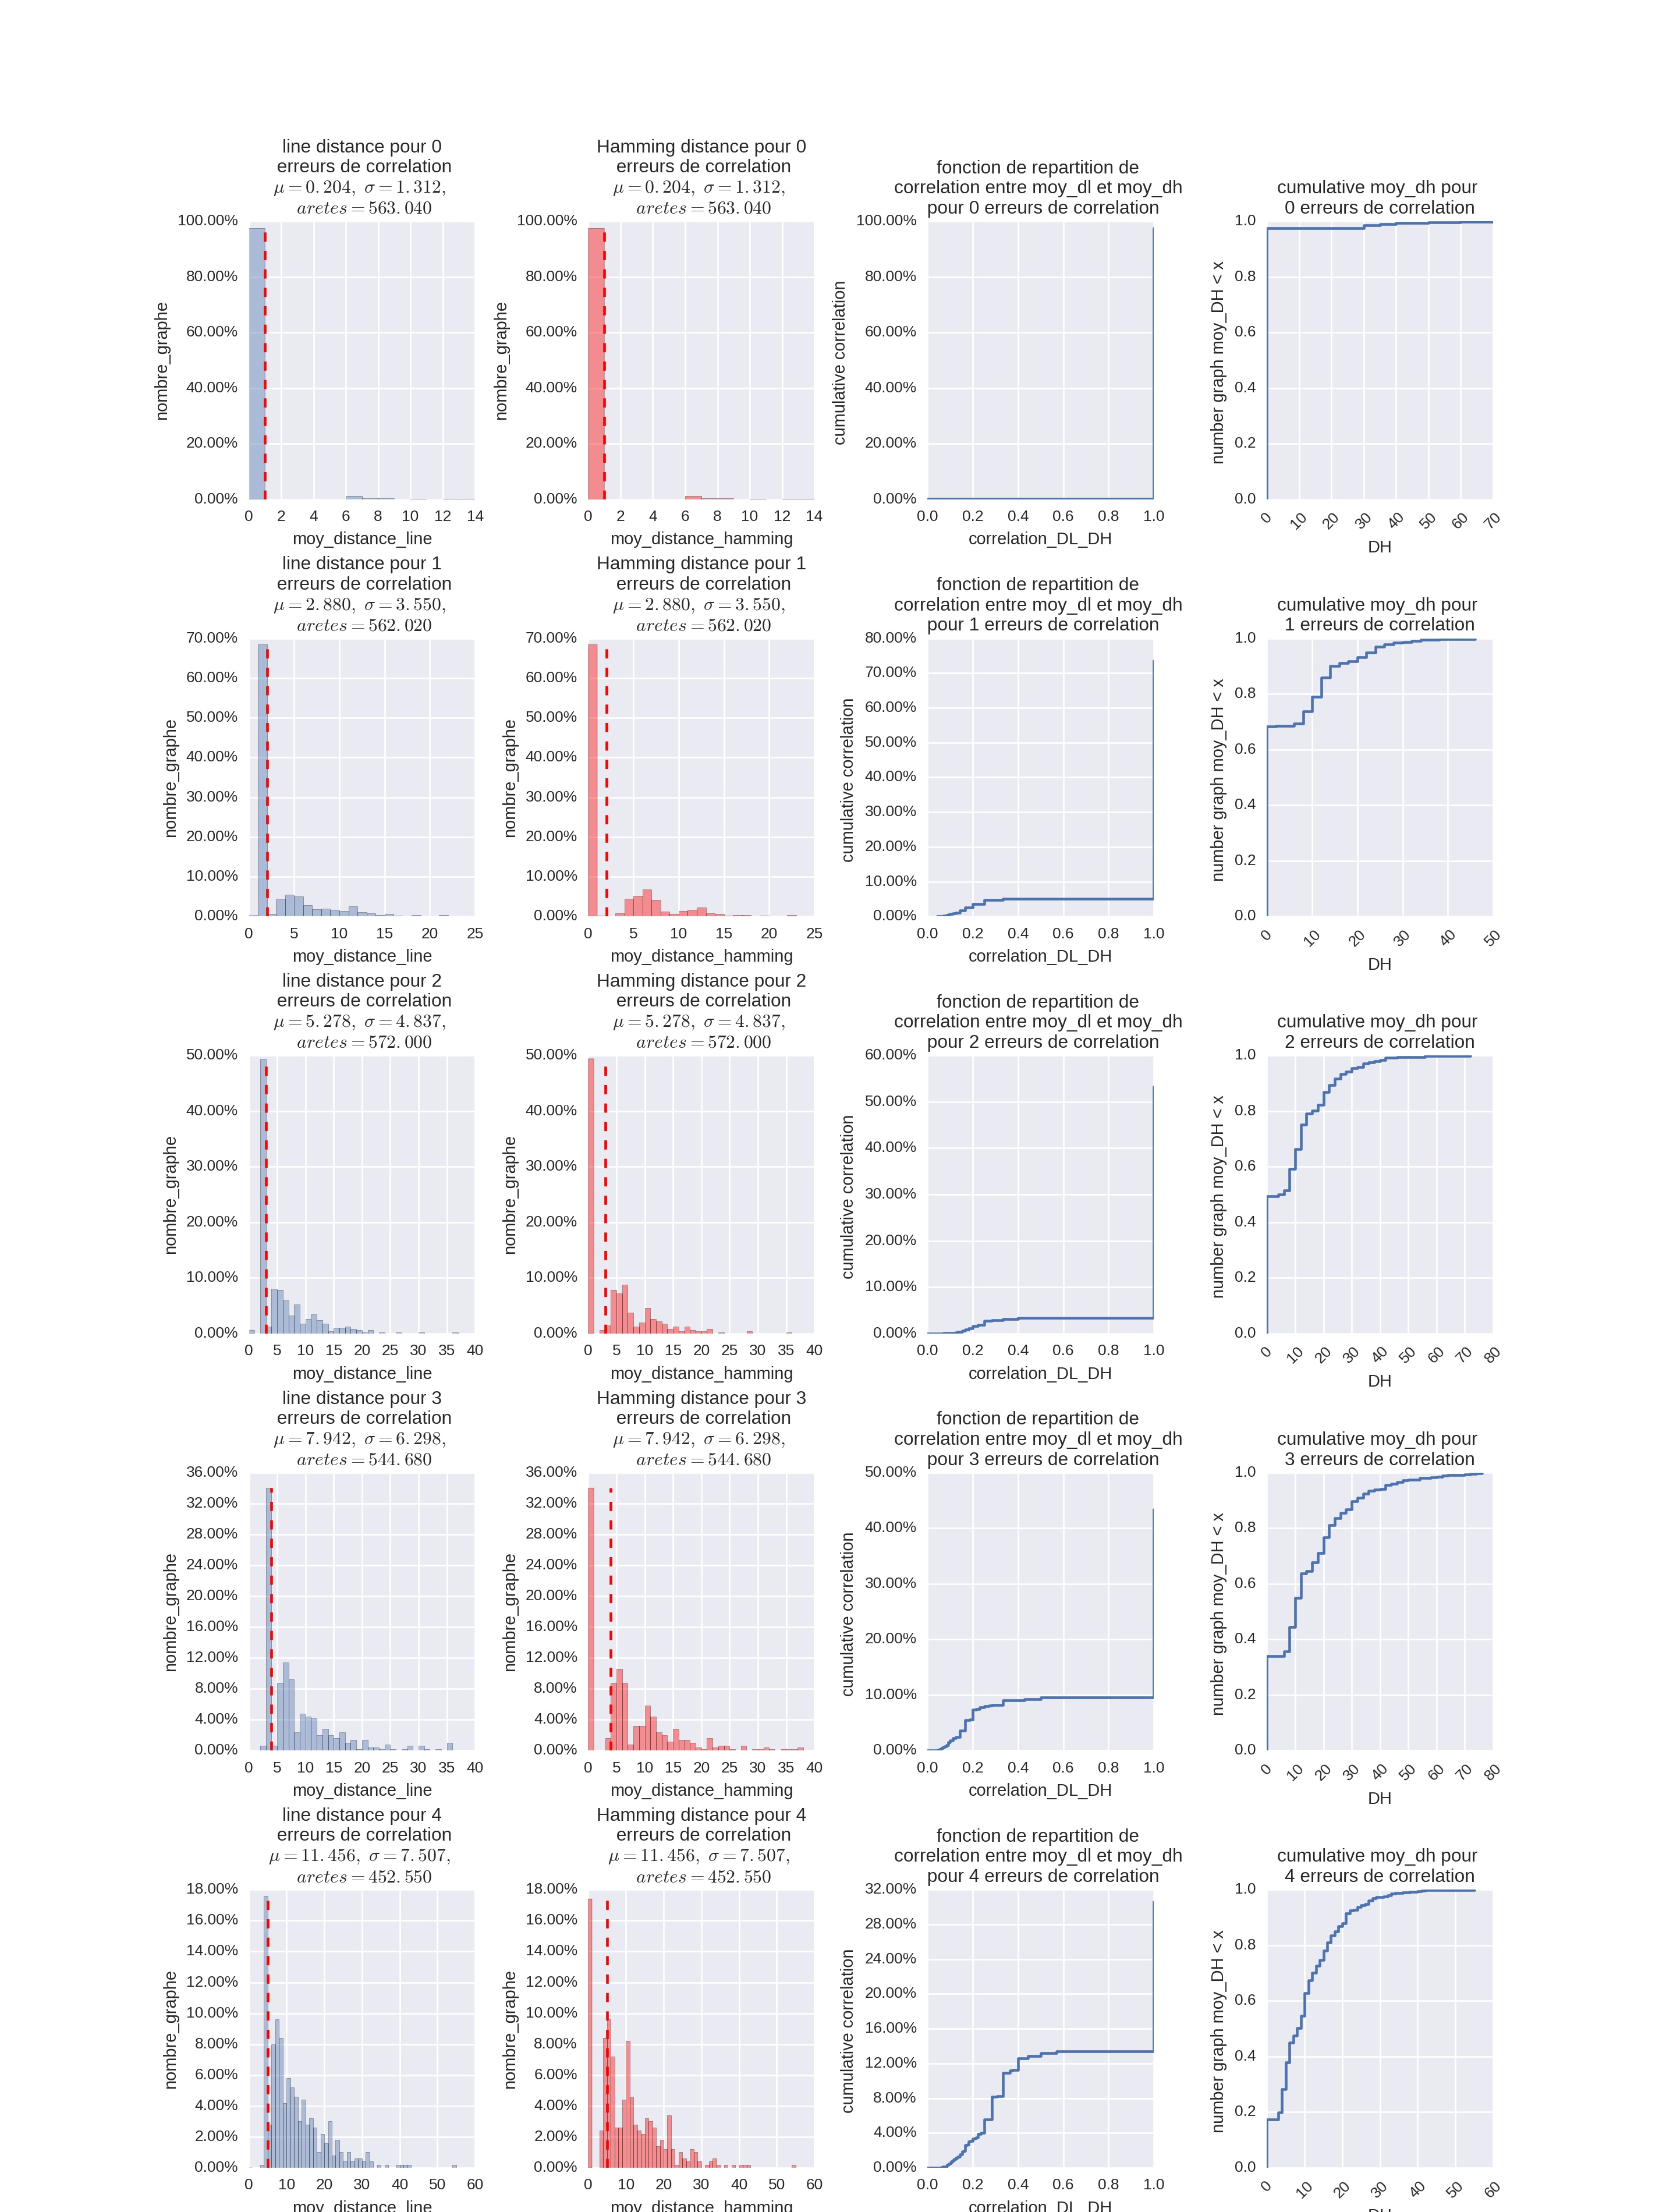
\includegraphics[scale=0.150]{permut_distanceMoyenDLDH_k_0_4_aleatoire_p_05.jpeg}
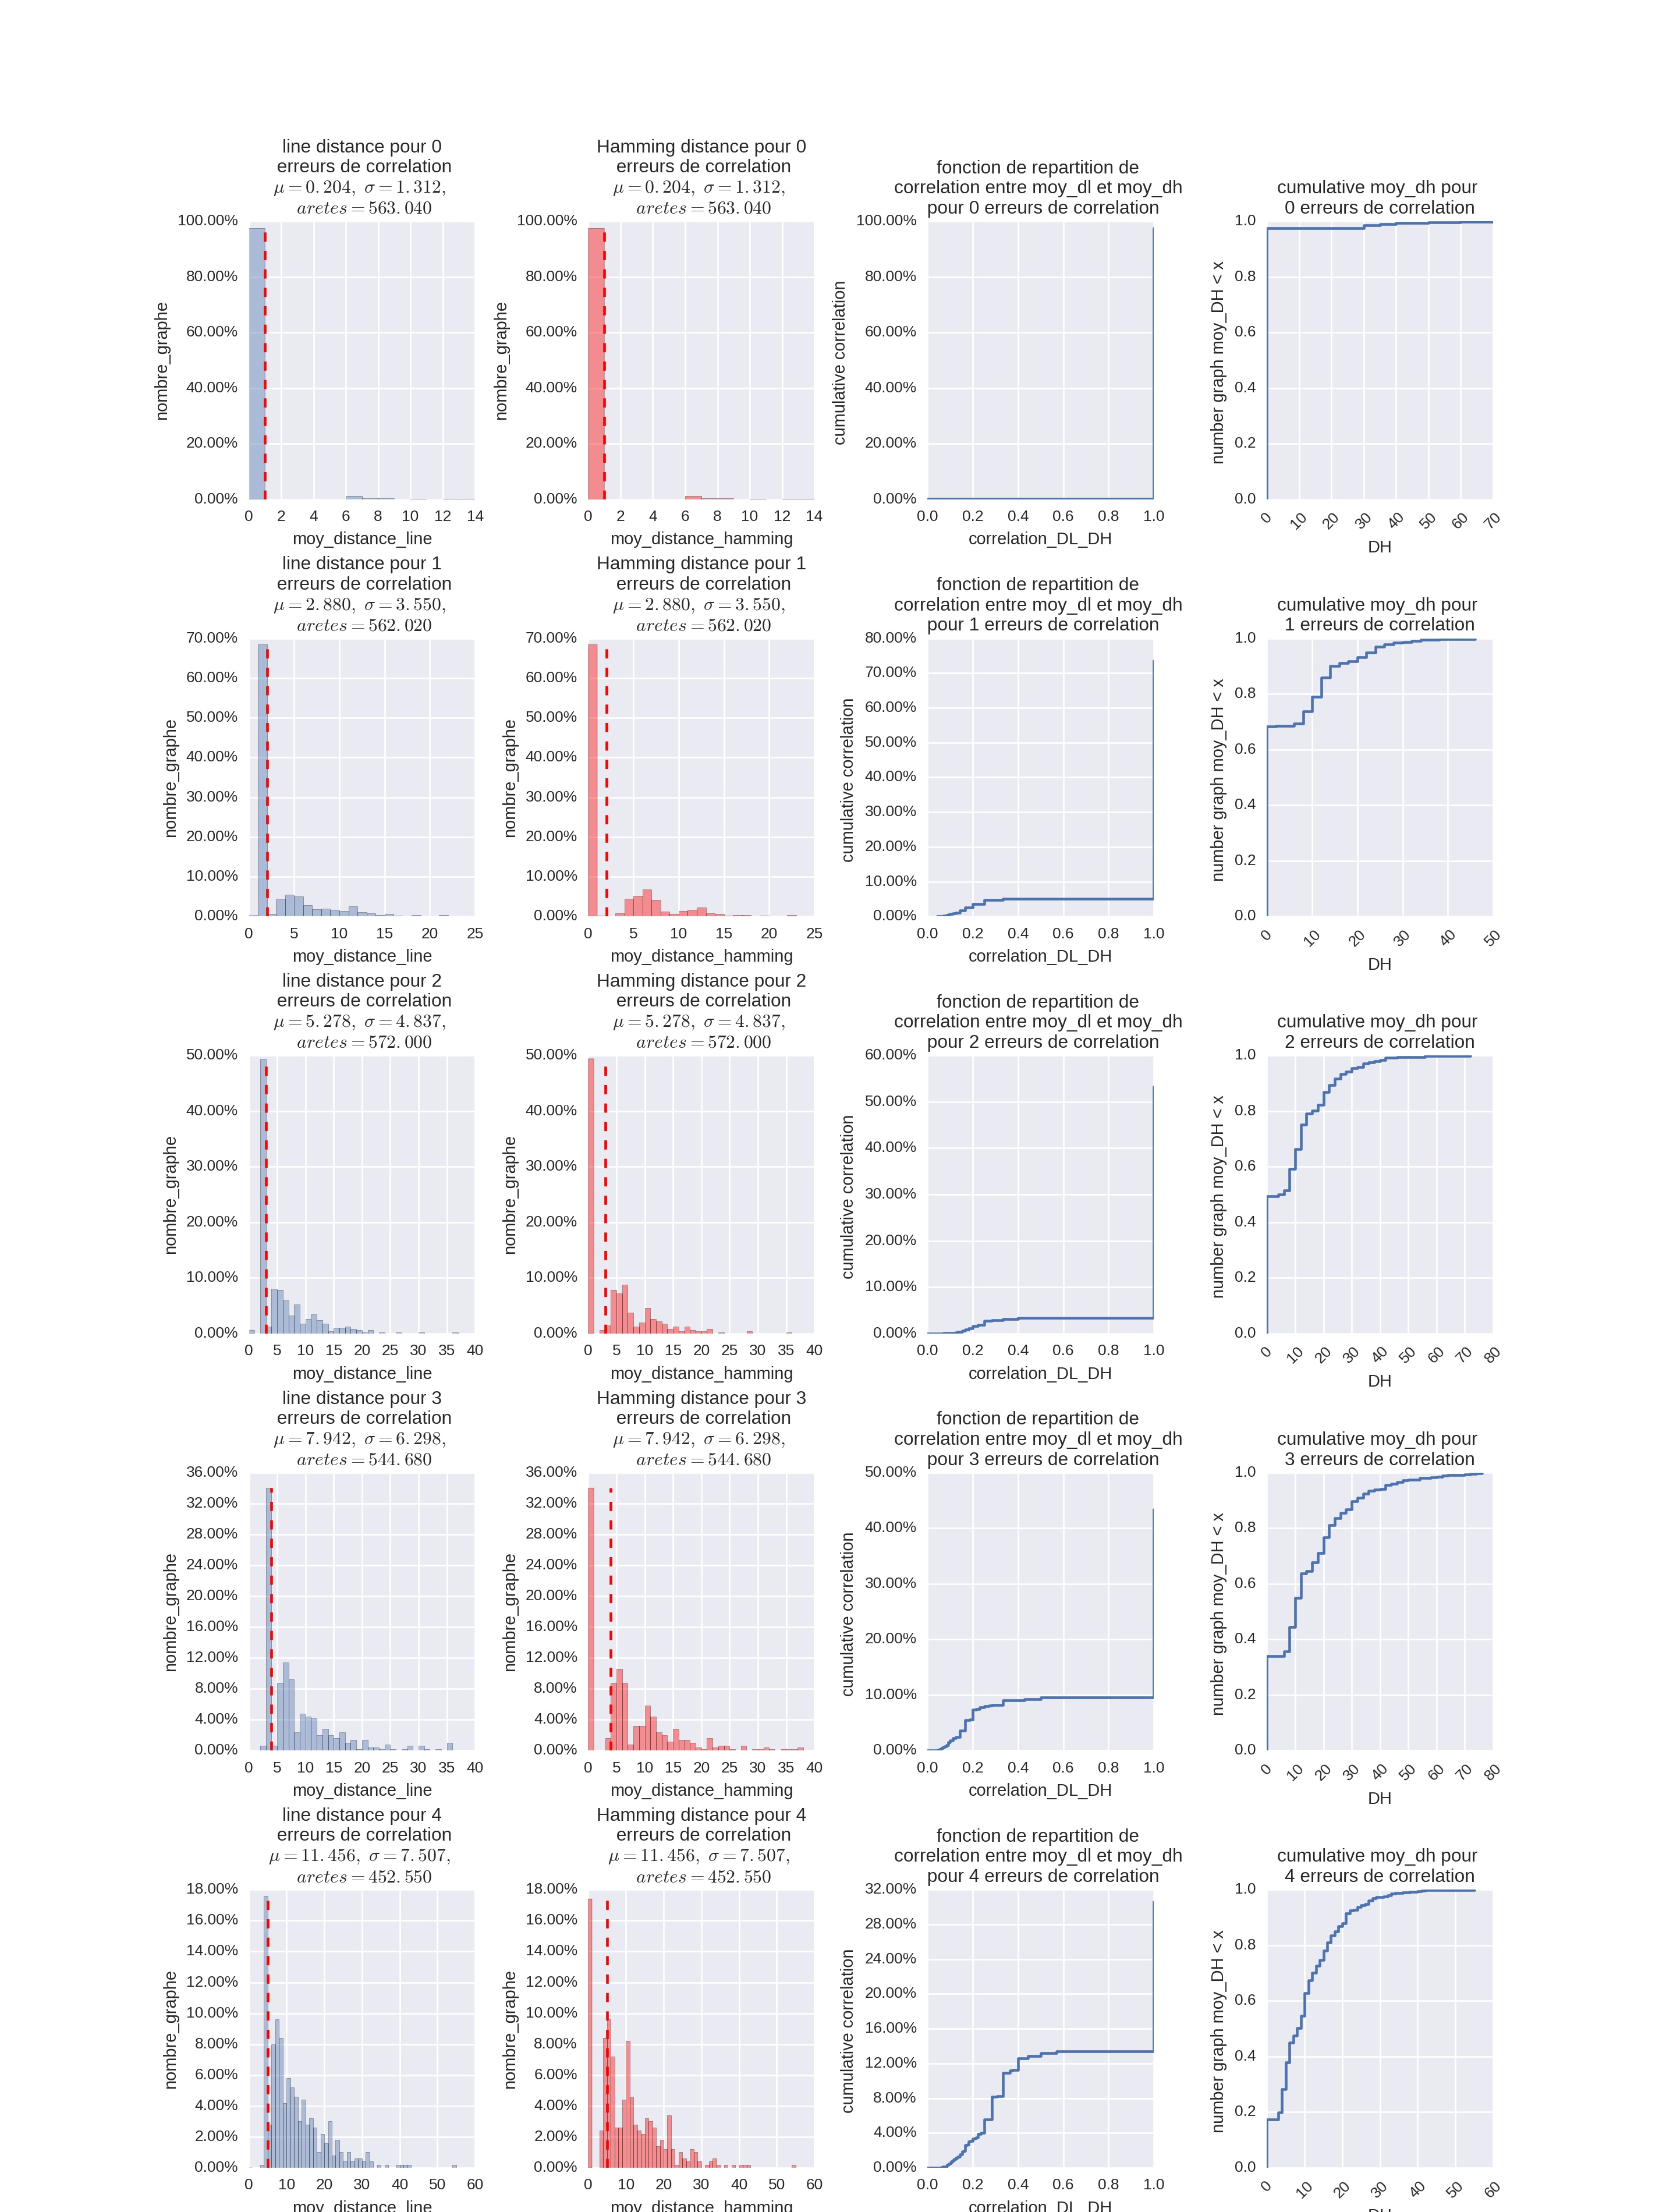
\includegraphics[width=550pt, height=600pt]{permut_distanceMoyenDLDH_k_0_4_aleatoire_p_05.jpeg}
\caption{ M\'ethode de permutation al\'eatoire avec une fonction de correction \`a co\^ut unitaire : distribution des distances line $moy\_DL$ et de Hamming $moy\_DH$ pour $k \in [0,  5]$ corr\'elations alter\'ees}
\label{permut_distanceMoyenDLDH_k_0_5_aleatoire_p_05} 
\end{figure}

\begin{figure}[htb!] 
\centering
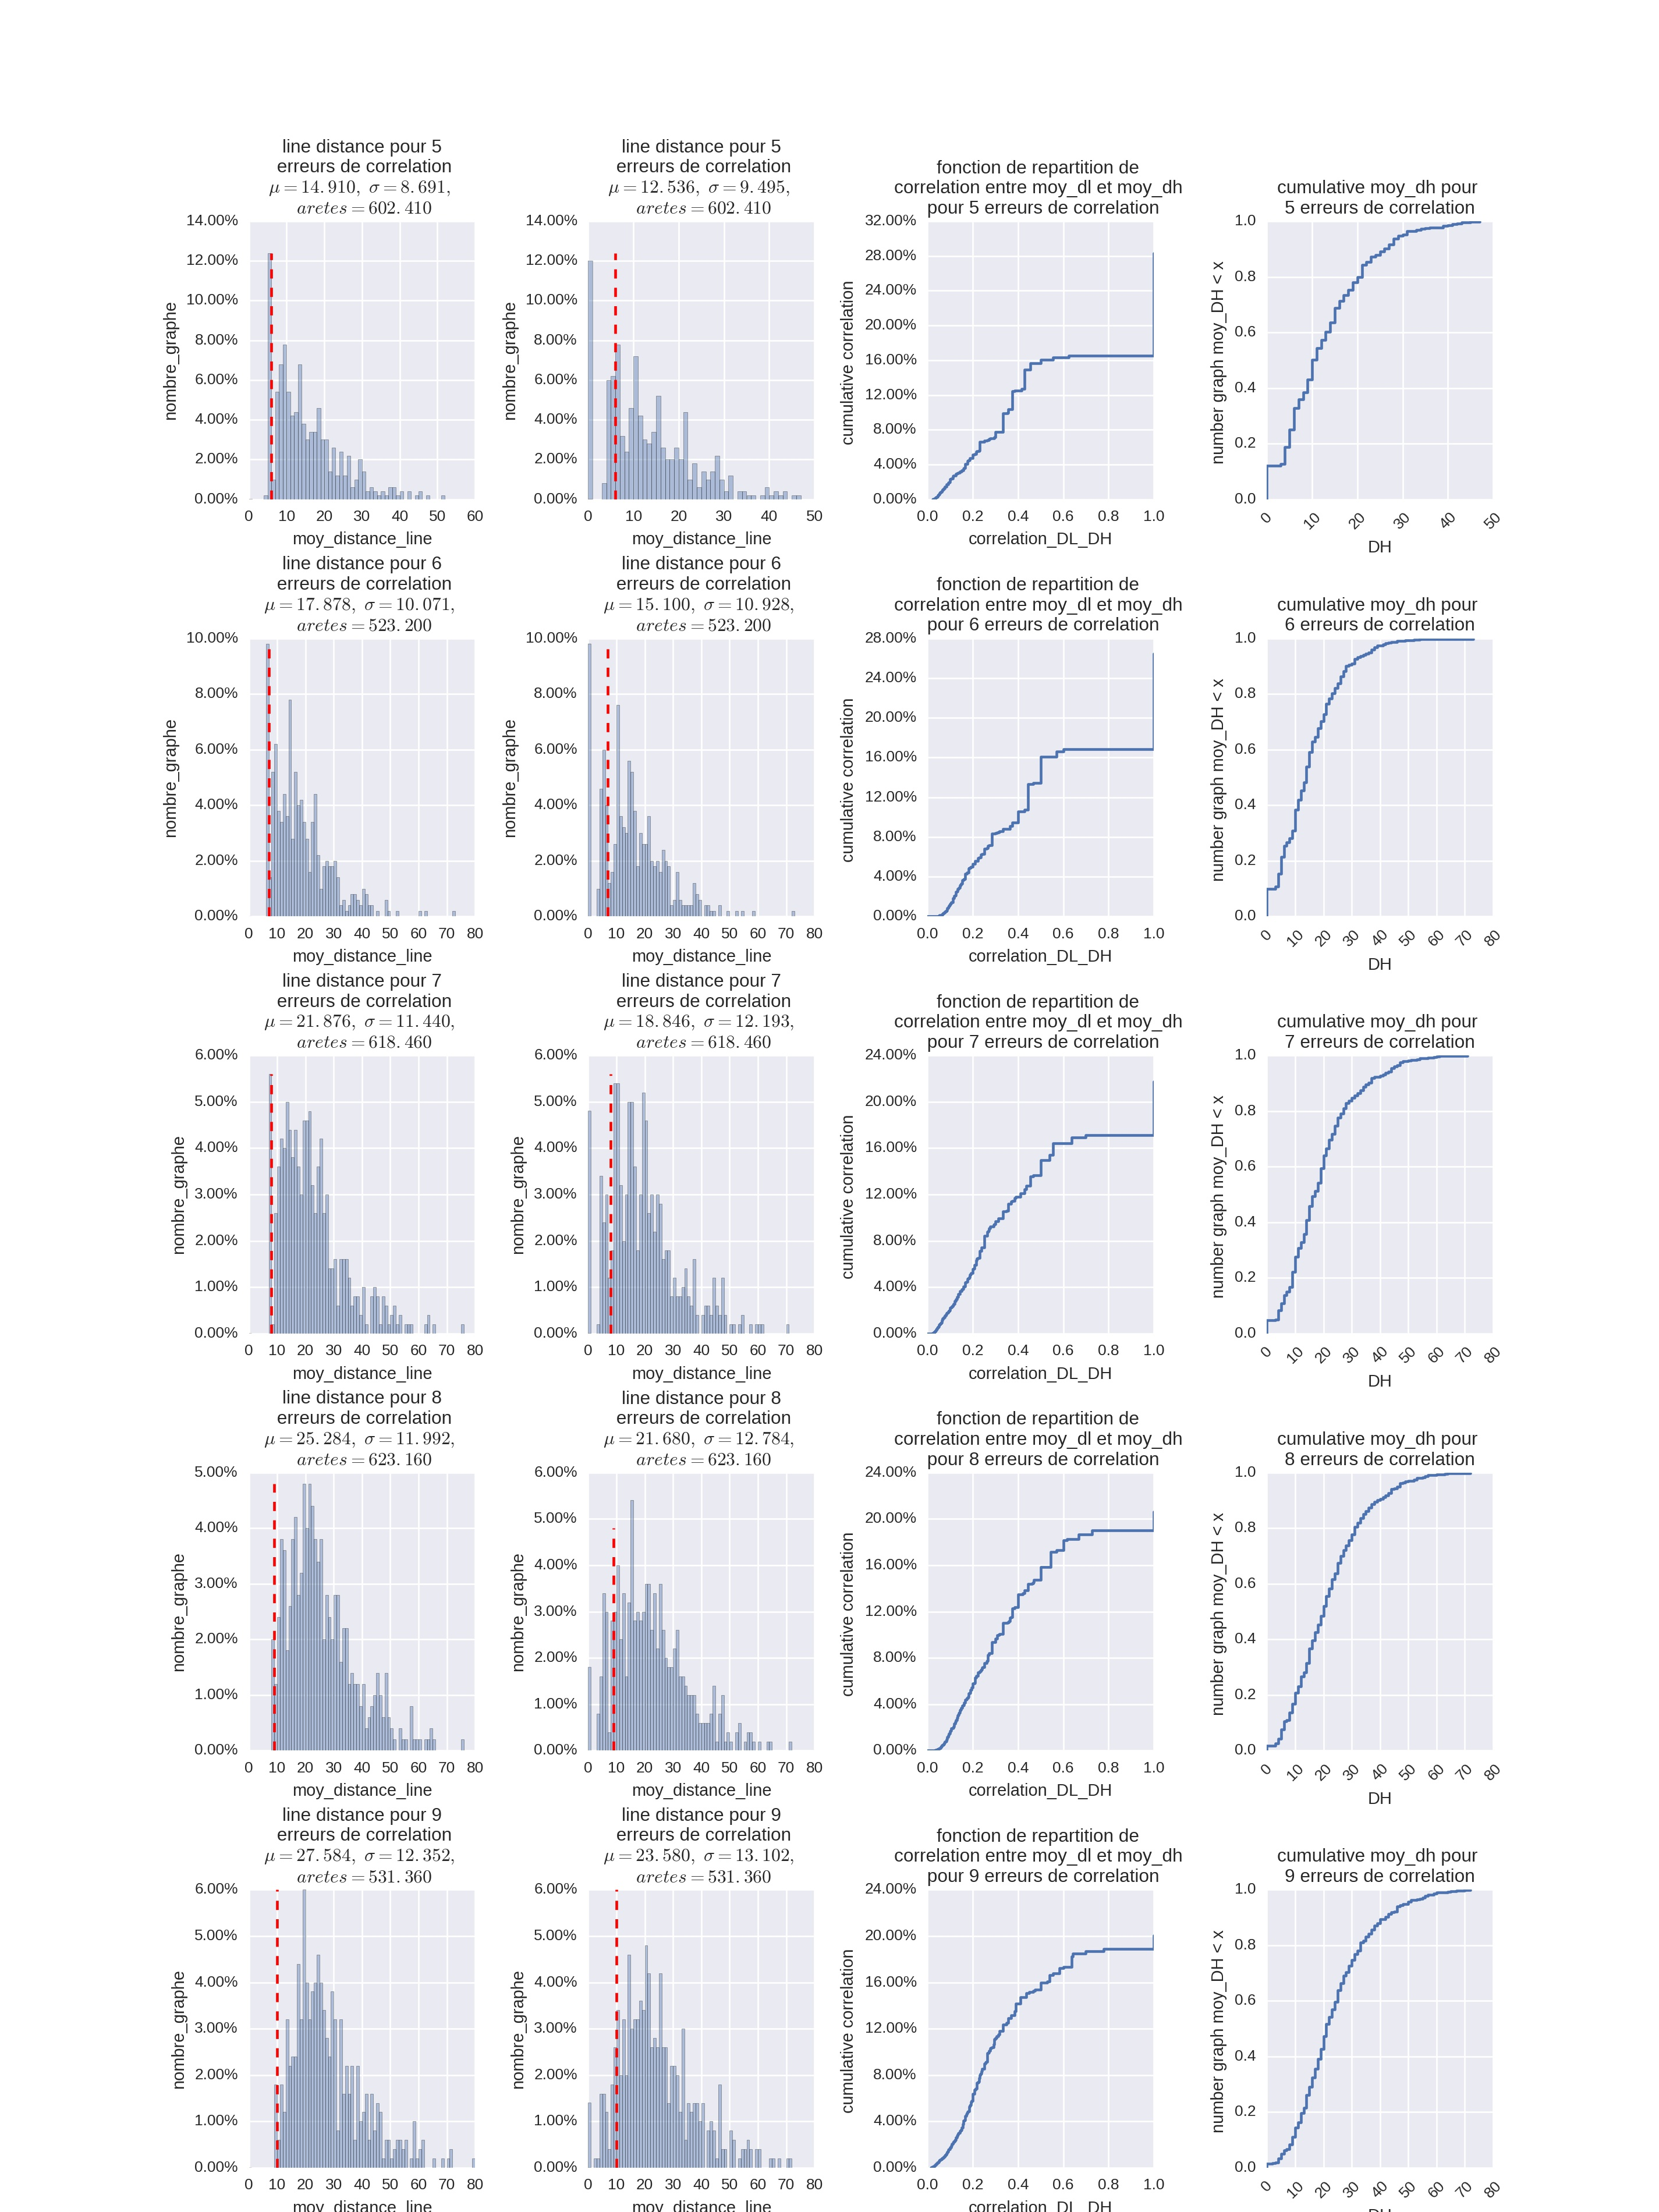
\includegraphics[width=550pt,height=600pt]{permut_distanceMoyenDLDH_k_5_9_aleatoire_p_05.jpeg}
\caption{ M\'ethode de permutation al\'eatoire avec une fonction de correction \`a co\^ut unitaire : distribution des distances line $moy\_DL$ et de Hamming $moy\_DH$ pour $k \in [6,  9]$ corr\'elations alter\'ees}
\label{permut_distanceMoyenDLDH_k_5_9_aleatoire_p_05} 
\end{figure}


La figure \ref{permut_distanceMoyenDLDH_k_0_5_aleatoire_p_05} repr\'esente les distributions des distances line, de Hamming, des fonctions de r\'epartition de la corr\'elation entre distances line et Hamming pour $k \in [0,5]$ erreurs. \newline
Pour $k=0$ erreur, nous avons un batonnet sur les histogrammes de distances line et de Hamming. Ce batonnet est le pourcentage d'ar\^etes identiques entre les graphes $G_k$ et $LG_k$ (distance line) et aussi entre les graphes  $LG$ et $LG_k$. Nous remarquons qu'un pourcentage de $100\%$ implique que les ar\^etes des graphes $LG_k$, d\'ecouvertes par les algorithmes, sont identiques \`a celle du graphe $LG$. Ce qui est normal parce que nous n'avons ajout\'e aucune erreur dans le line-graphe $LG$. Les courbes des fonctions de r\'epartition  suivent l'\'equation \ref{eqCorrelMoyDLDH} pour la corr\'elation entre les distances line et de Hamming et l'\'equation \ref{eqCumulMoyDH} pour la distance de Hamming.
\begin{equation}
\label{eqCorrelMoyDLDH}
y = \left\{
	\begin{aligned}
	0 \hspace{1 em} si \hspace{1 em} x < 1 \\
	100  \hspace{1 em}  si  \hspace{1 em}  x = 1
	\end{aligned}
	\right.
\end{equation}
\begin{equation}
\label{eqCumulMoyDH}
y = 1  \hspace{1 em}  si  \hspace{1 em}   x \in [0,1]
\end{equation}
Nous nous servirons du cas de $k=0$ erreur comme une r\'ef\'erence de la meilleure performance de nos algorithmes.
\newline
Pour $k \in [1,4]$, l'ensemble des batonnets, regroup\'es avant la droite $y = k$ (droite en rouge) de chaque histogramme, a un pourcentage sup\'erieure \`a $50 \%$. La pr\'esence de cette droite nous indique que, dans le majorit\'e des cas,  qu'il existe une diff\'erence de $k$ ar\^etes entre les graphes $G_k$ et $LG_k$ (voir distance line figure \ref{permut_distanceMoyenDLDH_k_0_5_aleatoire_p_05}) et ces $k$ ar\^etes correspondent aux erreurs ajout\'ees dans la matrice d'adjacence $matE$ du line-graphe $LG$. Cela explique 
la distance de hamming de $0$ ar\^ete entre $LG$ et $LG_k$ et le pourcentage pour $0$ erreur est le pic de chaque histogramme (voir distance de Hamming figure \ref{permut_distanceMoyenDLDH_k_0_5_aleatoire_p_05}).
% ajouter les fonctions cumulatives

Au d\'el\`a de $k \ge 5$ erreurs, le pic de chaque histogramme baisse significativement quand $k$ augmente (voir distances line et de  Hamming figure \ref{permut_distanceMoyenDLDH_k_5_9_aleatoire_p_05}). Une explication est la pr\'esence d'ar\^etes erron\'ees dans les line graphes $LG_k$ propos\'es parce que la majorit\'e de ces line-graphes qui ont plus de $k$ ar\^etes diff\'erentes entre $LG_k$ et $G_k$ alors que ce nombre $k$ doit correspondre au nombre d'erreurs ajout\'ees dans le line-graphe $LG$. Il s'illustre parfaitement avec $k = 9$ erreurs dans la figure \ref{permut_distanceMoyenDLDH_k_5_9_aleatoire_p_05} o\`u on a moins de $13\%$ de line-graphes dont les ar\^etes sont identiques et les $87\%$ restants ont plus d'une  ar\^ete diff\'erente.
\newline
%-------
Par ailleurs, les fonctions de r\'epartition des corr\'elations entre distances line et de Hamming et celle de la distance de Hamming ont des courbes  qui s'eloignent de celle de $k = 0$ erreur. En effet, ces courbes se divisent en deux parties : une courbe croissante et une droite verticale (distance de Hamming) ou horizontale (distance line). 
Pour $k \in [1,4]$, dans les figures des distributions cumulatives des distances de Hamming (colonne 4 de la figure \ref{permut_distanceMoyenDLDH_k_5_9_aleatoire_p_05}), on remarque que la droite verticale pour $k$ erreurs baisse quand $k$ augmente. Cette droite est le pourcentage de line-graphes identiques ($LG$ et $LG_k$). Par exemple, on a $69\%$ de line-graphes $LG_k$ identiques \`a $LG$ pour $k = 1$ alors qu'on en a que $19\%$ pour $k=4$. Cela est d\^u \`a l'ajout d'ar\^etes dans $LG_k$ n'appartenant pas \`a $LG$. Il se  forme une courbe exponentielle croissante dans laquelle on a plus de $10$ ar\^etes diff\'erentes pour $k \le 5$.  \newline
De m\^eme, au d\'el\`a du nombre d'ar\^etes diff\'erentes c'est-\`a-dire $moy\_DH > k$, nous constatons une droite verticale tr\`es courte qui baisse \'egalement quand la variable $moy\_DH$ augmente. Cela signifie qu'il y a tr\`es peu de line-graphes $LG_k$ ayant des  distances de Hamming tr\`es \'elev\'ees par rapport aux $k$ erreurs (voir figures \ref{permut_distanceMoyenDLDH_k_0_5_aleatoire_p_05} et \ref{permut_distanceMoyenDLDH_k_5_9_aleatoire_p_05})  pour $k \ge 5$.
\newline
Le fait que les distributions de distance line et de Hamming soient, toutes les deux, asym\'etriques (pour $k \le 6$) soient sym\'etriques (pour $k>6$) nous interrogent sur l'\'evolution des distributions des distances line par rapport \`a celles de Hamming. 